\section{Testen von Software und Systemen}\label{sec:testenSoftware}

Softwaretests sind in der heutigen Zeit eine wichtige Grundlage im Bereich der Qualitätssicherung bei Softwareprojekten. Abhängig von Komplexität und Sicherheitsanforderungen werden meist zwischen 30 und 60 Prozent der Kosten einer Software für die Qualitätssicherung und somit das Testen der Software verwendet \cite{Polo2013}. Ohne Softwaretests hätte heutige Software zahlreiche Fehler. Um die Wichtigkeit von Sofwaretests zu unterstreichen sieht \zB das V-Modell (vgl. \autoref{abb:v-modell}) für jeden Entwicklungsschritt am Ende eine entsprechende Testphase vor, woher auch der Name V-Modell stammt.

\begin{figure}
	\centering
	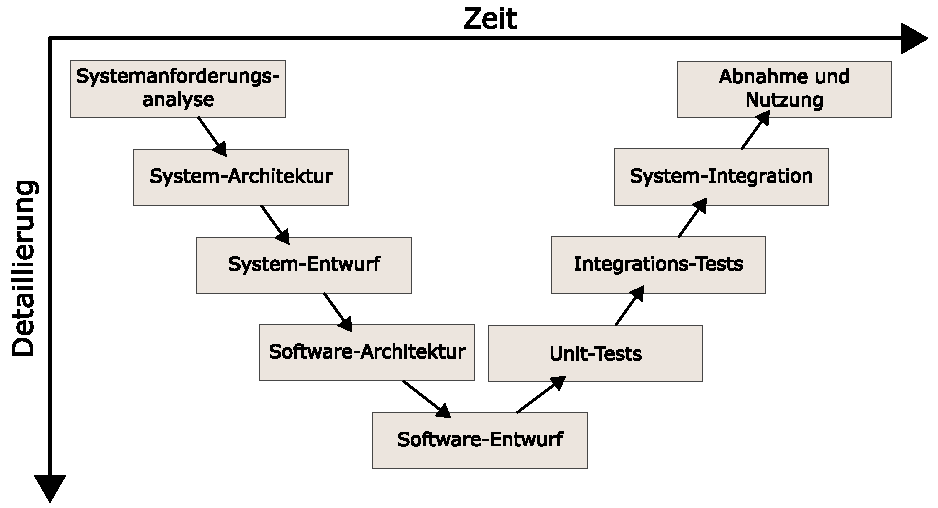
\includegraphics[width=0.8\textwidth]{./images/V-Modell.pdf}
	\caption[Aufbau des V-Modells]{Aufbau des V-Modells \cite{abb:vmodell}}
	\label{abb:v-modell}
\end{figure}

Nun ist es natürlich sehr aufwändig und daher mit einem vertretbaren Aufwand kaum machbar, jeden Test manuell durchzuführen. Daher wird versucht, möglichst viel zu automatisieren. Vor allem bei Unit-Tests ist dies mithilfe des \emph{XUnit}-Framework sehr einfach möglich. Dabei werden zunächst einzelne Testfälle erstellt und können im Anschluss aufgrund der aktuellen Codebasis jederzeit ausgeführt werden. Automatisierte Tests können auch dazu genutzt werden, um einen einzelnen Test mit verschiedenen Eingaben durchzuführen. Dadurch können verschiedene Eingabeklassen (wie negative oder positive Ganzzahlen) mit sehr geringem Aufwand in einem Test genutzt werden und somit verschiedene Testfälle direkt ausgeführt werden. Durch diese Testautomatisierung können somit zahlreiche Kosten eingespart werden.

Weitere Testframeworks gibt es auch zum Testen von sicherheitskritischen Systemen, welche nicht immer reine Software sein müssen. Dies ist einer der wichtigsten Anwendungsfälle für sogenannte \emph{Model Checker} (MC). \emph{Model Checking} (MC) wird dazu verwendet, um ein Modell auf seine Spezifikation zu testen. Dazu werden abhängig von den aktivierten Komponentenfehlern verschiedene Zustände des Modells vollautomatisch ausgeführt und anhand der dadurch im System auftretenden Fehler entschieden, ob die Spezifikation erfüllt wird (vgl. \autoref{sec:modelchecking}) \cite{Grumberg1999,Habermaier2015}.